\documentclass[a4paper, 12pt]{report}

\usepackage[italian]{babel}
\usepackage{graphicx}
\usepackage{float}
\usepackage{tabularx}
\usepackage{ltablex}
\usepackage[font=small,format=plain,labelfont=bf,up,textfont=normal,up,justification=justified,singlelinecheck=false,skip=0.01\linewidth]{caption}
\usepackage{enumitem}
\renewcommand{\familydefault}{\sfdefault}

\title{Assignment 2 - Programmazione di reti\newline Anno accademico 2018-2019}
\date{\today}

\author{Matteo Castellucci - 0000825436\\Elena Rughi - 0000832797\\Yuqi Sun - 0000826197\newline}

\begin{document}

\maketitle
\tableofcontents

\chapter{Task Uno}

\begin{figure}[H]
	\centering
	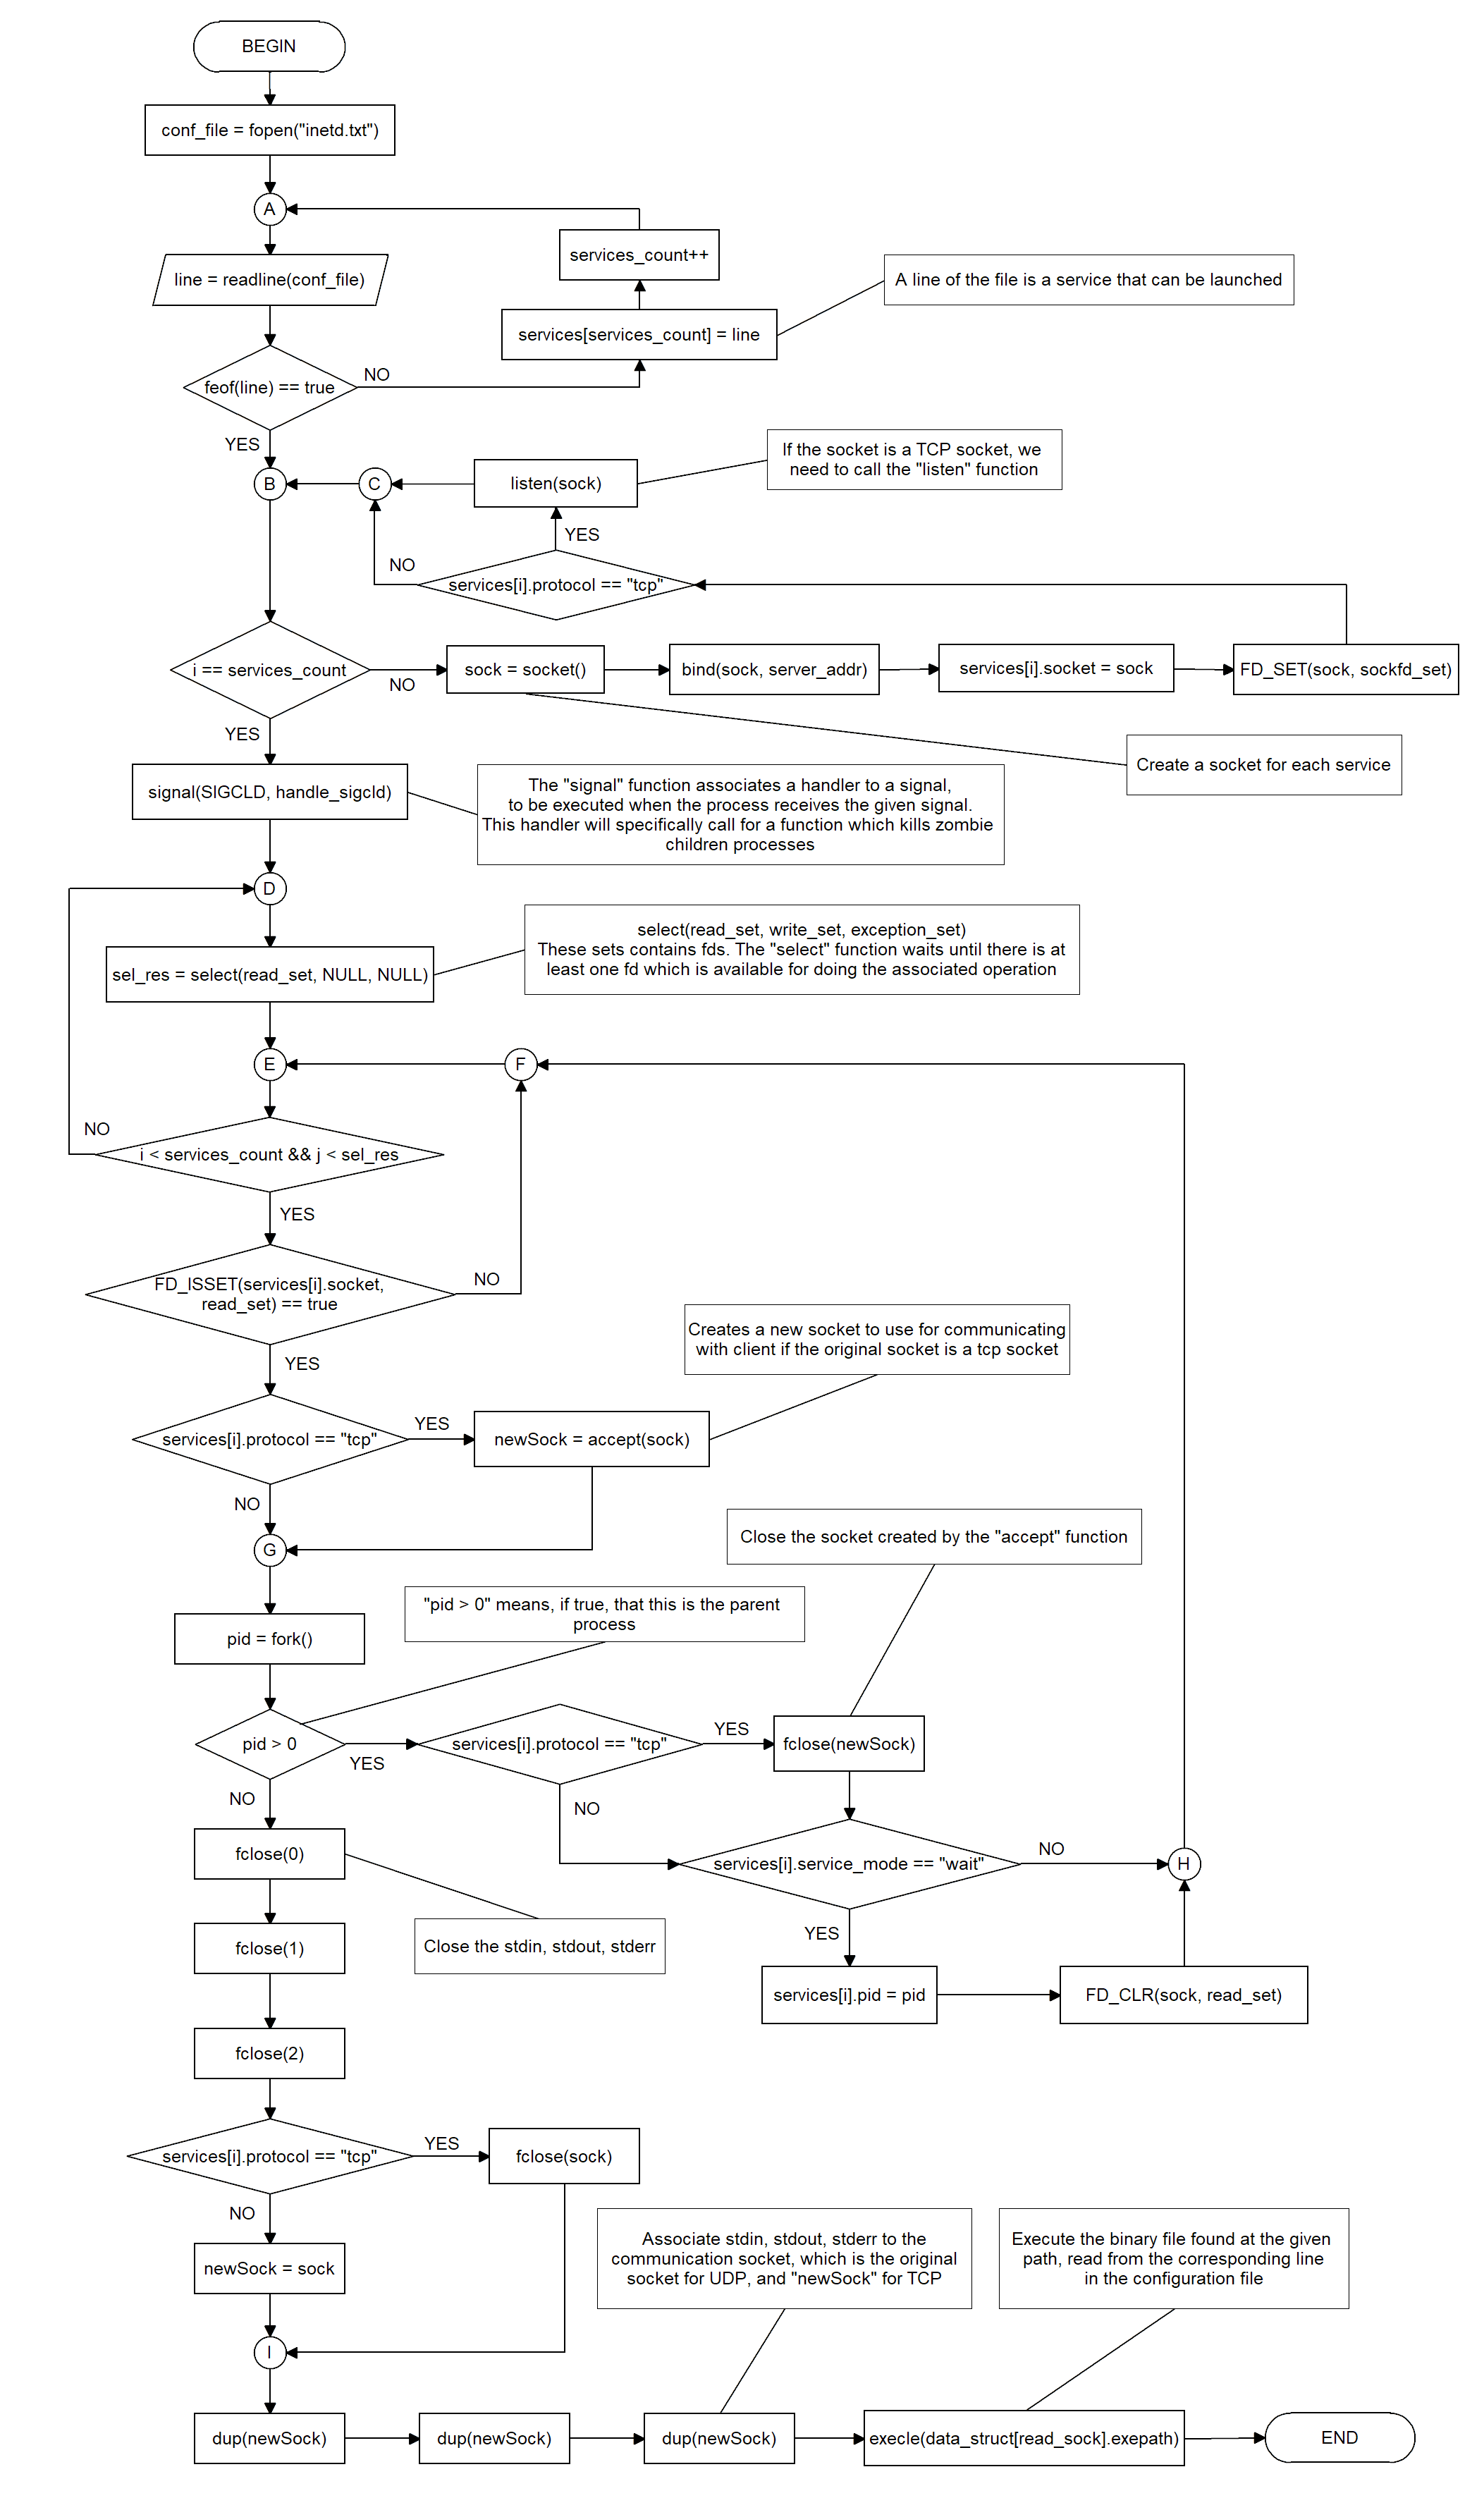
\includegraphics[width=\linewidth]{images/diagram.png}
	\caption{Diagramma di flusso seguito nel programma scritto}
\end{figure}

Questo scherma rappresenta il flusso di controllo seguito dal programma, così come indicato nelle slide. Lo schema segue lo standard ISO 5807 per i diagrammi di flusso. Sono presenti
sotto forma di operazioni tutte le \textit{system call} utilizzate, nonchè le macro per la gestione dei \textit{set} di \textit{file descriptor}. Per ciascuna delle prime è stato inserito
un commento che ne espliciti il funzionamento.

\chapter{Task Due}

\section{Design del ``\textit{superserver}"}

\begin{itemize}
    \item Inizialmente viene definita la struttura dati sotto forma di ``\textit{struct}" per ospitare tutte le informazioni necessarie per gestire un generico servizio
    \item Viene aperto il file ``inetd.txt" e viene letto riga per riga
    \item Ogni riga del file ha lo stesso formato di quattro parole: ``$<$percorso servizio$>$ $<$protocollo$>$ $<$porta$>$ $<$modalità servizio$>$". Queste informazioni vengono tutte
    memorizzate in una cella di un vettore di ``\textit{struct}" definite come sopra. Si tiene traccia del numero di servizi salvati
    \item Viene inizializzato il \textit{set} dei ``\textit{socket file descriptor}" associati ai servizi salvati e viene creata una \textit{socket} per ogni servizio tramite le
    funzioni necessarie: ``\textit{socket}", ``\textit{bind}", anche ``\textit{listen}" nel caso la socket fosse di associata al protocollo \textit{TCP}. La \textit{socket}
    viene salvata assieme ai dati del servizio corrispondente nel vettore di ``\textit{struct}" nonchè viene inserita nel \textit{set} indicato precedentemente
    \item Viene registrato l'\textit{handle} per il segnale di morte di un processo figlio, ``\textit{SIGCHLD}". In questo modo, ogni volta che un processo figlio muore,
    se si occupava di gestire le richieste per un servizio in modalità ``\textit{wait}", si preoccupa di renderlo disponibile per i \textit{client} successivi che vogliono
    accedervi reinserendolo nel \textit{set} dei ``\textit{socket file descriptor}"
    \item La parte finale si basa su un ciclo che viene eseguito senza condizione di uscita, dove all'inzio si ha la funzione ``\textit{select}". Questa permette al
    \textit{superserver} di rimanere in stato di \textit{wait} finchè almeno una socket è pronta per essere letta, ovvero un \textit{client} vuole comunicare con il
    \textit{superserver}. Si trova in un ciclo perchè alla presenza di un segnale mandato al processo che esegue il programma, si interrompe l'attesa della funzione mentre
    si vuole invece continuare ad attendere per i \textit{client}
    \item Allo scattare della ``\textit{select}", per ogni ``\textit{socket}" pronta, si controlla se è necessario usare la funzione ``\textit{accept}" se essa è di tipo
    \textit{TCP}. Dopodichè, si crea un processo figlio mediante la \textit{system call} ``\textit{fork}"
    \item Il processo figlio è responsabile di chiudere ``\textit{stdin}", ``\textit{stdout}" e ``\textit{stderr}" e sostituirli, mediante la \textit{system call ``dup"},
    con una \textit{socket}. Se il suo tipo è \textit{UDP}, la \textit{socket} scelta per la sostituzione è quella nel vettore di ``\textit{struct}", altrimenti se è di tipo \textit{TCP}
    quella scelta è la \textit{socket} restituita dalla funzione ``\textit{accept}", mentre quella nel vettore viene chiusa. Infine, il processo figlio sostituisce il proprio
    eseguibile binario con quello del servizio richiesto mediante la funzione ``\textit{execle}"
    \item Nel frattempo, il processo padre, qualora la socket pronta fosse di tipo \textit{TCP}, chiude la \textit{socket} per la comunicazione creata dalla funzione ``\textit{accept}".
    In seguito, in caso il servizio richiesto fosse avesse modalità ``\textit{wait}", rimuove dal \textit{set} dei ``\textit{socket file descriptor}" la socket appena entrata in
    uso. In questo modo, nessuno potrà più richiedere quel servizio fino a che l'utilizzo da parte del \textit{client} corrente non sarà terminato. 
\end{itemize}

\section{Compilazione del ``\textit{superserver}"}

È stato utilizzato il ``\textit{Makefile}" incluso assieme agli altri file di questo assignment.

\section{Descrizione dei test effettuati per controllare il comportamento del ``\textit{superserver}"}

.Compilazione di tutti i file sorgente, come specificato sopra
		.Esecuzione da terminale del superserver
		.Per ogni test (udp wait e nowait, tcp wait e nowait) esecuzione di 2 processi client
		.Uso del comando bash "ps -aux" per visualizzare i processi in esecuzione,
		 per osservare il numero di processi attivi dei server avviati dal superserver
		.L'indirizzo IP passato come argomento all'esecuzione del processo client adottato è 
		 l'indirizzo di loopback 127.0.0.1 (identificato tramite il comando ifconfig)
		.Il numero di porta passato come argomento all'esecuzione del processo client
		 deve corrispondere alle indicazioni del file inetd.txt

\section{Comportamento del ``\textit{superserver}"}

1) what's the behaviour of udpServer in wait mode? and in no wait mode?
		
			udpServer, wait: è in esecuzione un solo server udp, che è in grado di
			comunicare con diversi client, in quanto il server attende il completamento
			dell'operazione corrente prima di iniziarne una nuova; il server quindi
			adempie le richieste di molteplici client in modo sequenziale tramite
			un unico processo.
			
			udpServer, nowait: in questo caso, se più di un client si connette al server,
			il server crea molteplici processi al fine di soddisfare le richieste
			di ogni client.
			
		2) what's the behaviour of tcpServer in wait mode? and in no wait mode?
			
			tcpServer, wait: quando più client tentano di connettersi al server, esso
			interagisce con un client alla volta; a differenza del server udp,
			poichè il protocollo udp necessita dell'instaurazione di una connessione
			con un client, il server non può interagire con altri client finchè ha una
			connessione attiva, pertanto il server crea un solo processo.
			Infatti dopo la terminazione del primo processo client, il server si connette
			al secondo ed esegue le richieste di quest'ultimo.
		
			tcpServer, nowait: il server quando riceve molteplici richieste di connessione da
			parte di diversi client crea un processo per ogni client, così da poter
			interagire con essi contemporaneamente.

\end{document}
